\documentclass[tikz,border=3mm]{standalone}
\usepackage{amsmath}
\usetikzlibrary{arrows.meta,calc,positioning}

\begin{document}
\pagecolor{white}
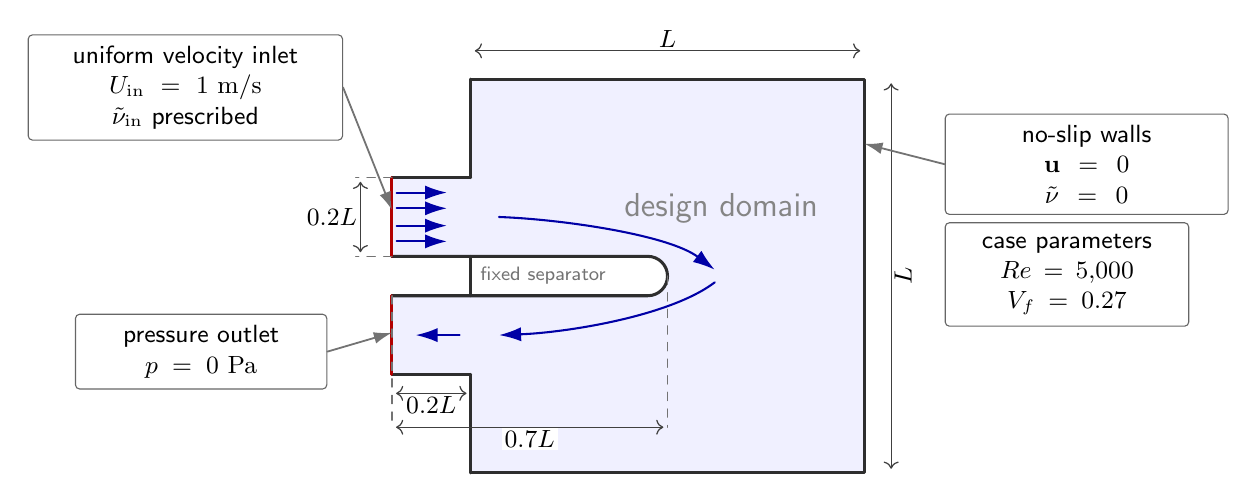
\begin{tikzpicture}[
  line cap=round,
  line join=round,
  font=\sffamily\small,
  flow/.style={-{Latex[length=2.8mm,width=1.8mm]}, line width=0.75pt, draw=blue!65!black},
  dim/.style={<->, line width=0.45pt, draw=black!75, shorten <=1.5pt, shorten >=1.5pt},
  bc/.style={draw=black!60, fill=white, rounded corners=1.5pt, inner xsep=7pt, inner ysep=4pt, align=center},
  wall/.style={draw=black!82, line width=1.1pt},
  boundary/.style={draw=red!70!black, line width=1.1pt},
  guide/.style={draw=black!55, dashed, line width=0.45pt},
  dimlabel/.style={fill=white, inner sep=1pt, font=\sffamily\small},
  designlabel/.style={font=\sffamily\large, text=black!48}
]

\def\L{5.0}
\def\lead{1.0}
\def\topLow{2.75}
\def\topHigh{3.75}
\def\topMid{3.25}
\def\botLow{1.25}
\def\botHigh{2.25}
\def\botMid{1.75}
\def\barLow{2.25}
\def\barHigh{2.75}
\def\barCenterY{2.50}
\def\barRectEnd{2.25}
\def\barTipX{2.50}
\def\barRadius{0.25}

% Design and non-design fluid regions.
\fill[blue!6] (0,0) rectangle (\L,\L);
\fill[blue!6] (-\lead,\topLow) rectangle (0,\topHigh);
\fill[blue!6] (-\lead,\botLow) rectangle (0,\botHigh);
\node[designlabel] at (3.18,3.36) {design domain};

% Fixed separator.
\fill[white] (-\lead,\barLow) -- (\barRectEnd,\barLow)
  arc[start angle=-90,end angle=90,radius=\barRadius] -- (-\lead,\barHigh) -- cycle;
\draw[wall] (-\lead,\barLow) -- (\barRectEnd,\barLow)
  arc[start angle=-90,end angle=90,radius=\barRadius] -- (-\lead,\barHigh);
\node[font=\sffamily\scriptsize, text=black!55, fill=white, inner sep=1pt] at (0.92,\barCenterY)
  {fixed separator};

% No-slip external walls.
\draw[wall] (0,\L) -- (\L,\L) -- (\L,0) -- (0,0);
\draw[wall] (0,0) -- (0,\botLow);
\draw[wall] (0,\botHigh) -- (0,\topLow);
\draw[wall] (0,\topHigh) -- (0,\L);
\draw[wall] (-\lead,\topHigh) -- (0,\topHigh);
\draw[wall] (-\lead,\topLow) -- (0,\topLow);
\draw[wall] (-\lead,\botHigh) -- (0,\botHigh);
\draw[wall] (-\lead,\botLow) -- (0,\botLow);

% Boundary sections.
\draw[boundary] (-\lead,\topLow) -- (-\lead,\topHigh);
\draw[boundary] (-\lead,\botLow) -- (-\lead,\botHigh);

% Uniform inlet velocity and flow path around the separator.
\foreach \y in {2.94,3.14,3.36,3.56}{
  \draw[flow] (-0.94,\y) -- (-0.30,\y);
}
\draw[flow] (0.36,\topMid) .. controls (1.18,3.22) and (2.52,3.02) .. (3.10,2.58);
\draw[flow] (3.10,2.42) .. controls (2.52,1.98) and (1.18,1.78) .. (0.36,\botMid);
\draw[flow] (-0.14,\botMid) -- (-0.70,\botMid);

% Dimensions.
\draw[dim] (0,5.36) -- node[dimlabel, above] {$L$} (\L,5.36);
\draw[dim] (5.34,0) -- node[dimlabel, midway, rotate=90, below] {$L$} (5.34,\L);

\draw[guide] (-\lead,\topHigh) -- (-1.46,\topHigh);
\draw[guide] (-\lead,\topLow) -- (-1.46,\topLow);
\draw[dim] (-1.40,\topLow) -- node[dimlabel, left] {$0.2L$} (-1.40,\topHigh);

\draw[dim] (-\lead,\botLow-0.24) -- node[dimlabel, below] {$0.2L$} (0,\botLow-0.24);
\draw[guide] (-\lead,\barLow) -- (-\lead,0.58);
\draw[guide] (\barTipX,\barCenterY) -- (\barTipX,0.58);
\draw[dim] (-\lead,0.58) -- node[dimlabel, below] {$0.7L$} (\barTipX,0.58);

% Boundary-condition labels.
\node[bc, anchor=south east, text width=35mm] (inletLabel) at (-1.62,4.22)
  {uniform velocity inlet\\$U_{\mathrm{in}}=1~\mathrm{m/s}$\\$\tilde{\nu}_{\mathrm{in}}$ prescribed};
\draw[-{Latex[length=2.3mm,width=1.5mm]}, black!55, line width=0.65pt]
  (inletLabel.east) -- (-\lead,3.34);

\node[bc, anchor=east, text width=27mm] (outletLabel) at (-1.82,1.54)
  {pressure outlet\\$p=0~\mathrm{Pa}$};
\draw[-{Latex[length=2.3mm,width=1.5mm]}, black!55, line width=0.65pt]
  (outletLabel.east) -- (-\lead,1.78);

\node[bc, anchor=west, text width=31mm] (wallLabel) at (6.02,3.92)
  {no-slip walls\\$\mathbf{u}=0$\\$\tilde{\nu}=0$};
\draw[-{Latex[length=2.3mm,width=1.5mm]}, black!55, line width=0.65pt]
  (wallLabel.west) -- (5.00,4.18);

\node[bc, anchor=west, text width=26mm] at (6.02,2.52)
  {case parameters\\$Re=5{,}000$\\$V_f=0.27$};

\end{tikzpicture}
\end{document}
